\chapter{Architectural Viewpoint}
For this project we have chosen to make use of the \emph{4+1 view model}, where we have put most ephasis on the \emph{Logic}, \emph{Development} and \emph{Process} views.

    \section{Logic View}
    \textbf{Purpose:} In the Logic View we decompose the functional requirements into different classes and show the relationship between these requirements. This in order to showcase the functionality that the system provides to the end users.

    
    
    \noindent\textbf{Stakeholders:} Course staff, ATAM evaluators and Developers 
    
    
    \begin{figure}[h]
        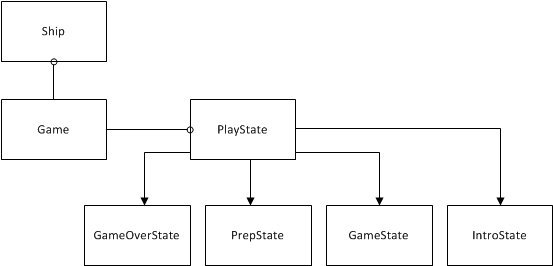
\includegraphics[width=\textwidth]{LogicalView.png}
        \caption{UML Class diagram illustrating the Logical View}
        \label{fig:LogicalView}
    \end{figure}


    Figure \ref{fig:LogicalView} shows a simplified overview of the different classes, usages and object inheritances. Notation is based on the Logical View notation by Kructhen\cite{kruchten}. This decomposition helps identify elements that are shared across the system.

    \texttt{GameOverState}, \texttt{PrepState}, \texttt{GameState} and \texttt{IntroState} all extend a common \texttt{PlayState} class, and describes the different states the game can exist in at a given time.

    The main \texttt{Game} class functions as the game's main controller, and controls the state stack. The \texttt{Ship} object instantiates the different ship types with a given set of attributes, which in turn is controlled by the main \texttt{Game} class.

    Other states and objects are discussed earlier in this report, but are not represented in this diagram. The main reason for this descision is to keep the diagram simple and easy to read, and that the ignored features are either redundant or too specific.



    \section{Development view}
    \textbf{Purpose:} In the development view we illustrate how the different parts of the system looks a developers perspective. Different parts of the system is divided into layers. This view supports allocation of requirement
    and work to developers and also monitoring project progress.  
    
    \noindent\textbf{Stakeholders:} Course staff, ATAM evaluators and Developers
    

    \begin{figure}[h]
        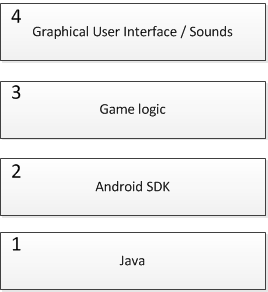
\includegraphics{DevelopmentView.png}
        \caption{Development View Architecture Layer Diagram}
        \label{fig:DevelopmentView}
    \end{figure}
    
    
    
    \section{Process view}
    \noindent\textbf{Purpose:} In the process view we illustrate how different tasks are combined into the final product. In the process view we consider performance and availability requirements, and also system integrity and fault tolerance.
    The process view can specify which thread of control executes operations in the classes identified in the logic view. 

    \noindent\textbf{Stakeholders:} Users, Course staff, ATAM evaluators and Developers 
    
    \begin{figure}[h]
        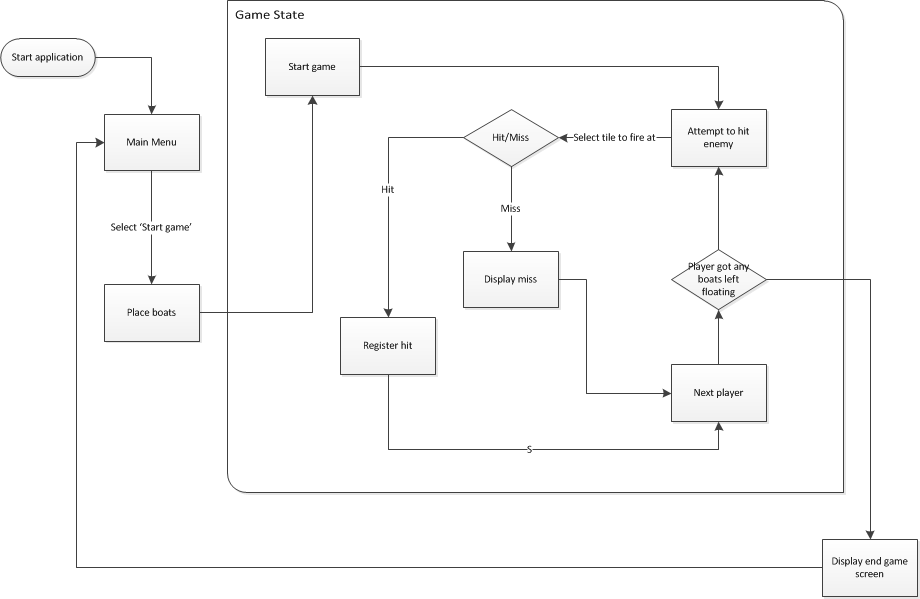
\includegraphics[angle=90, scale=0.8]{ProcessLayer.png}
        \caption{Process View Activity Diagram}
        \label{fig:DevelopmentView}
    \end{figure}